

\chapter{Implementation} \label{sec:implementation}

\section{System diagram}

Figure \ref{fig:system} can help the reader to gain understanding how each of the materials and methods used as described in Section \ref{sec:mm} fit together.

\begin{figure}[h!]
    \centering
    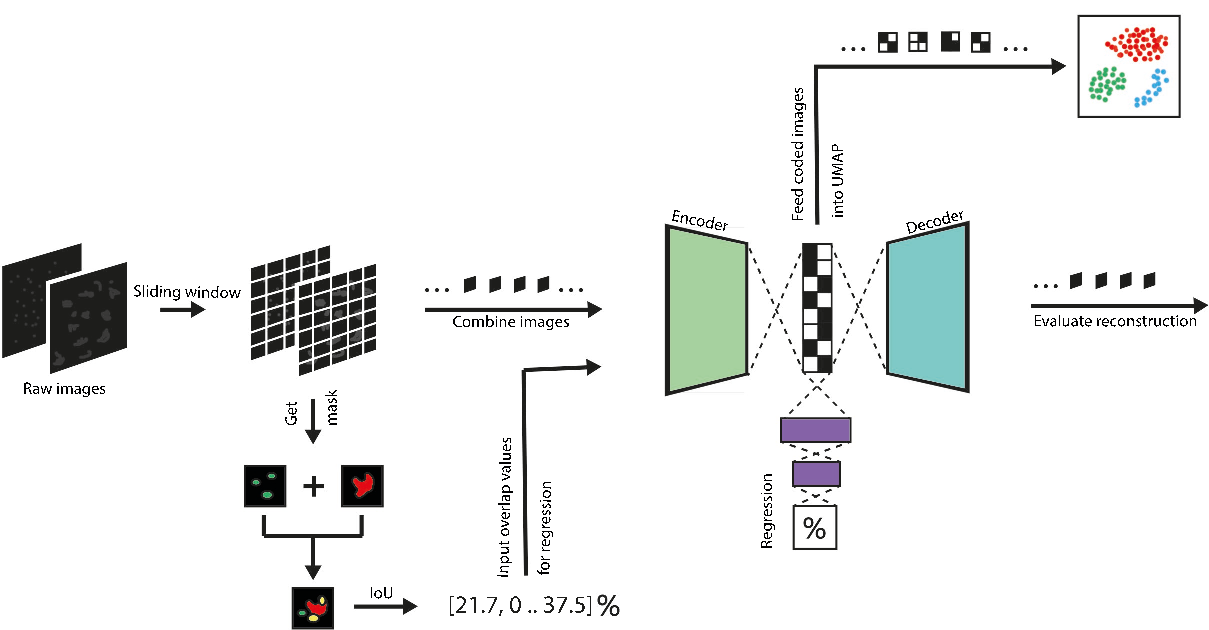
\includegraphics[width=\textwidth]{dissertation/figures/system_diagram.pdf}
    \caption{[TO ANNOTATE] System diagram showing how each image will be decomposed and analysed.}
    \label{fig:system}
\end{figure}

\section{Experimental setup}

As this is a research project based on using deep learning methods, a large part of the research involved an experimental process of tweaking the deep learning models, training them, and evaluating them.

\section{Pre-processing}

Firstly, before feeding them as input into any model, the images of cells had to be pre-processed. This is already partly discussed in Section \ref{}. This section will go over the implementation specifics.

\bigskip
The following list provides a step-by-step of the process:
\begin{enumerate}
    \item For each dataset, all the images of T cells and dendritic cells were picked out. Their corresponding filenames were retrieved.
    \item The filenames were sorted to keep images from the same well next to each other in memory.
    \item Each image was partitioned into sub-images through a sliding window approach. The window was of size 192x192 and yielded a 100 same-sized images. The original image was 2048x2048 so the right and bottom borders of the image were discarded.
    \item Once this gridded dataset was obtained, each T cell image was combined in a RGB image with its dendritic cell counterpart, stored in index i and index i+100 respectively.
    \item For each combined image, noise was removed through low value pixel clipping. Min-max normalisation was then applied to put all images in the same [0,1] range.
\end{enumerate}

Some implementation choices made in the above have to be justified.

\subsection{Sliding window size}

The sub-image window size was chosen to be 192x192 because of the way Pooling and Upsampling operations function in autoencoders. Autoencoders are built around symmetrical operations around a bottleneck. That is, we are trying to output a reconstructed image which will be of the same size as the input.

[make an image]
%Encoder layers in autoencoders make use of Pooling operations to reduce dimensionality of the input as you go deeper into the network. These pooling operations are commonly done in factors of 2 for their efficiency at downsizing as well as maintaining detail. In the context of an image passing through an autoencoder, it is reduced by 2 for every pooling operation. Each pooling operation then has a corresponding upsampling operation in the decoder part of the autoencoder, in order to reconstruct the image with the right size. An upsampling operation of factor 2 outputs an image of dimensions multiplied by 2. However, a pooling operation will round up resultant dimensions if the reduction of the original dimensions results in a decimal number. The corresponding upsampling operation would then double that number, which would result in a different dimension in the output of the autoencoder. Hence, we had to pick a size that would be big enough to show enough cells, but we also had to pick a size which meant the image could be divided by 2 for a large amount of times, depending on the number of hidden layers. To illustrate, if we apply a division by to the number 200 three times, the image can be upsampled and reconstructed correctly, however if it is reduced 4 times, then after the 4th operation we obtain a 13x13 image and the first upsampling operation creates a 26x26 image. A size which is a multiple of 8 bypasses that issue for a larger number of operations. A 192x192 image can be reduced 6 times, when it reaches dimensions of 3x3, without running into upsampling issues.

\subsection{Image combination}

Images of each type of cells on their own would not make much sense on their own when the aim is to quantify the level of interaction. Hence they have to be combined. The advantage that the provided dataset has is that it comes with the T cells and the dendritic cells separated by means of fluorescent dyes, hence no image segmentation technique had to be used to be able to separate the image out into the different types of cells and colour them in. Instead, each of the T cell and its corresponding DC, which were associated to the same file, were combined together in an RGB image, with the blue channel set to 0. %The images were not combined in an absolute difference operation as we would have lost information of where the images overlapped i.e. interacted, which is what we are looking into in this research.

\section{Quantifying immune cell interaction}

% To obtain an interaction measure from the images, multiple methods were explored. First, we looked at the Structural Similarity Index (SSIM) of images. was computed, however because the images were so similar in general i.e. white blobs spread across a black background, the results were extremely similar across all cells in different experiment conditions.

The idea was [instead] to obtain masks of the images and compute the intersection over union area as the interaction value. As the cells were bright blobs on a black background, and we did not have the task of separating T-cells from dendritic cells, it was hoped that this would be straightforward. Both K-means and thresholding methods yielded good results and their specifics are detailed below.

\subsection{\textit{k}-means colour clustering}

k-means has been shown to perform well on image segmentation by quantising the number of colours in an image into \textit{k} clusters. Formally, k-means aims to partition data points in an array into \textit{k} sets such that the variance between points within clusters is minimised. In our case we wanted to use k-means to transform our black-and-white images of immune cells into bichrome images that we could use as masks. [The following pseudocode details the process of K-means.]

\begin{algorithm}
    \DontPrintSemicolon
    \KwData{$I$, an array of pixel values making an image.\;
    $k$, the number of colours to partition the image's colour palette to.\;}
    \KwResult{A set of $k$ clusters.}
    \Begin{
        Initialise $k$ objects picked from $I$\;
        \While{clusters are still changing}
        {
           Assign each item $i$ in $I$ to the cluster with closest mean value\;
           Recompute the mean of each cluster\;
        }
    }

\caption{Pseudocode for the k-means algorithm applied to image segmentation.}
\label{alg:kmeans}
\end{algorithm}

k-means clustering is conveniently offered by multiple libraries in Python. We looked at both scikit-learn's and OpenCV's k-means. scikit-learn is a general library  for machine learning tools, while OpenCV is a more specialised library built for Computer Vision purposes. Both their k-means functions are straightforward to initialise and use. Their performance was benchmarked in order to select the best one. The table below reports times for k-means initialised with k=2, random initialisation of centroids and 10 iterations. The test was ran on a 2015 MacBook Pro with 2.7 GHz i5 core and 8 GB memory.

% Please add the following required packages to your document preamble:
% \usepackage{multirow}
\begin{table}[]
\centering
\begin{tabular}{|l|l|l|}
\hline
\textbf{Initialisation} & \textbf{OpenCV} & \textbf{Scikit-learn} \\ \hline
Random                                   & \multicolumn{1}{r|}{18.9s}       & \multicolumn{1}{r|}{165s}              \\ \hline
k-means++                                & \multicolumn{1}{r|}{29.3s}       & \multicolumn{1}{r|}{139s}              \\ \hline
\end{tabular}

\caption{CPU times for OpenCV's and scikit-learn's k-means tool ran on 1,000 samples of 192x192 pixels with different methods of initialising centroids.}
\end{table}

As we can see OpenCV outperforms scikit-learn in all cases. OpenCV for Python is a wrapper library around the original OpenCV code built in C++, which gives it a boost in performance. OpenCV's k-means was thus selected. Initially, k-means centers were initialised randomly. However, during training and validation it was found that this method of initialisation was yielding highly different results for the intersection over union metric at every run. Hence, some speed was traded for consistency and the kmeans++ center initialisation method was picked instead.

\subsection{Thresholding}

An alternative to k-means in the case of black-and-white images is thresholding. We decided to explore this option as it could have performance improvements compared to K-means.

Thresholding refers to the process of converting a grayscale image to a binary image of pixels. Pixels above a set threshold are set to 1, and the rest of the pixels below that threshold are set to 0. Thresholding depends on pixel distribution analysis. Usually, thresholding works well for images which have different peaks of pixel values in their distribution. However, in the case of our images we had one peak of pixel values. Figure \ref{fig:thresholdhist} illustrates this.

\begin{figure}[h]
    \centering
    \begin{subfigure}{0.45\textwidth}
        \centering
        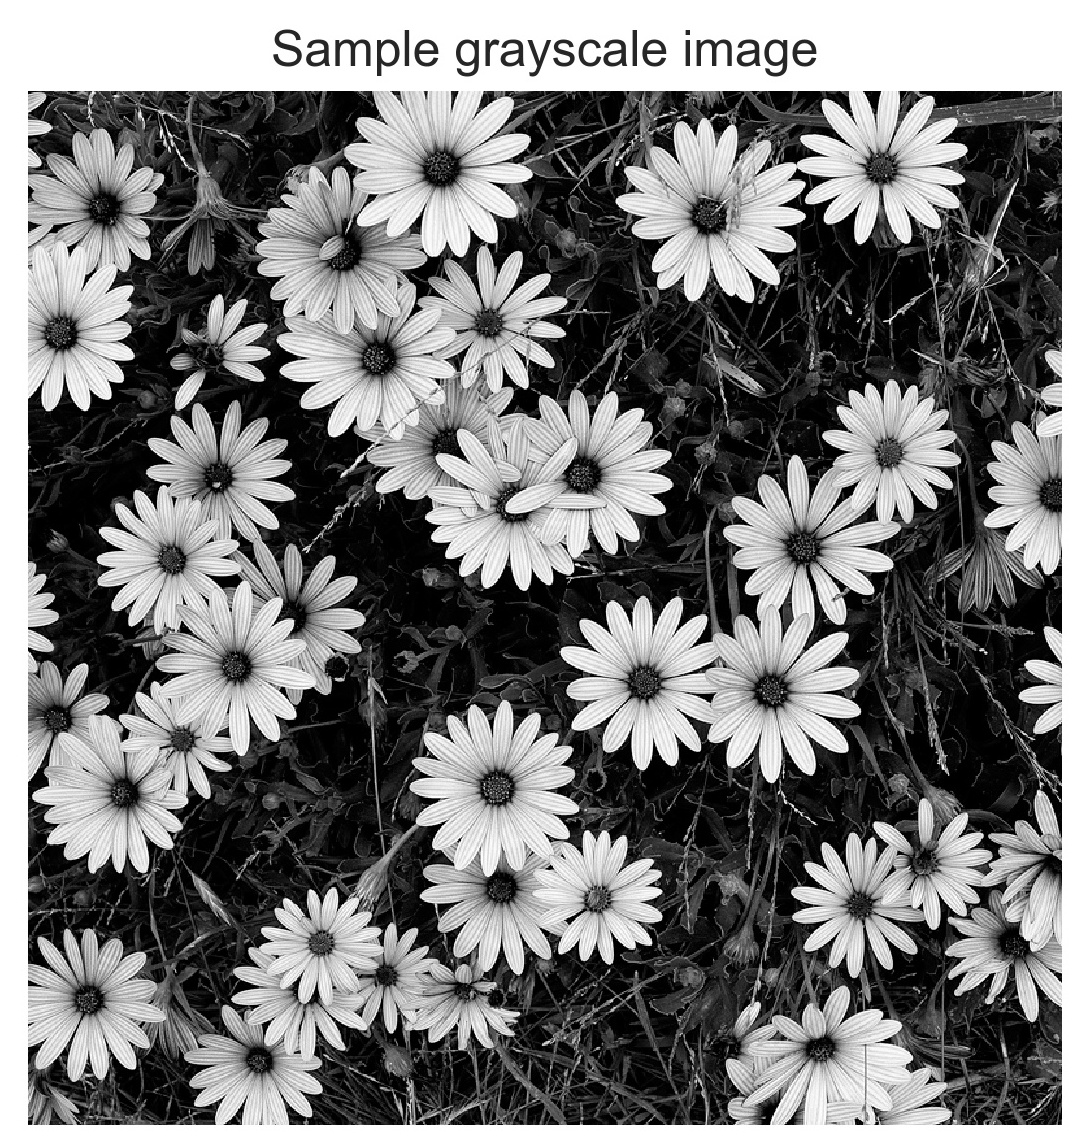
\includegraphics[width=.5\textwidth]{dissertation/figures/sample_grayscale.jpg}
    \end{subfigure}
    \begin{subfigure}{0.45\textwidth}
        \centering
        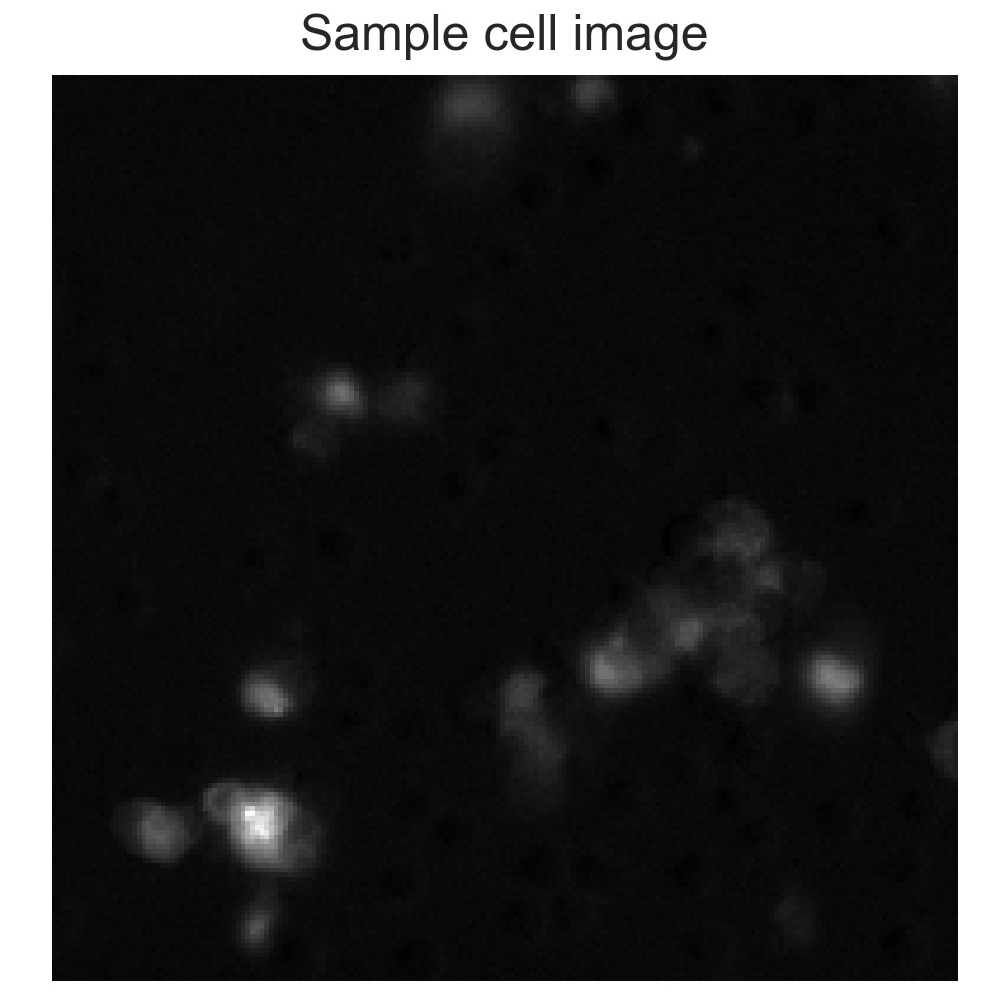
\includegraphics[width=.5\textwidth]{dissertation/figures/sample_cell.jpg}
    \end{subfigure}
    \begin{subfigure}{0.45\textwidth}
        \centering
        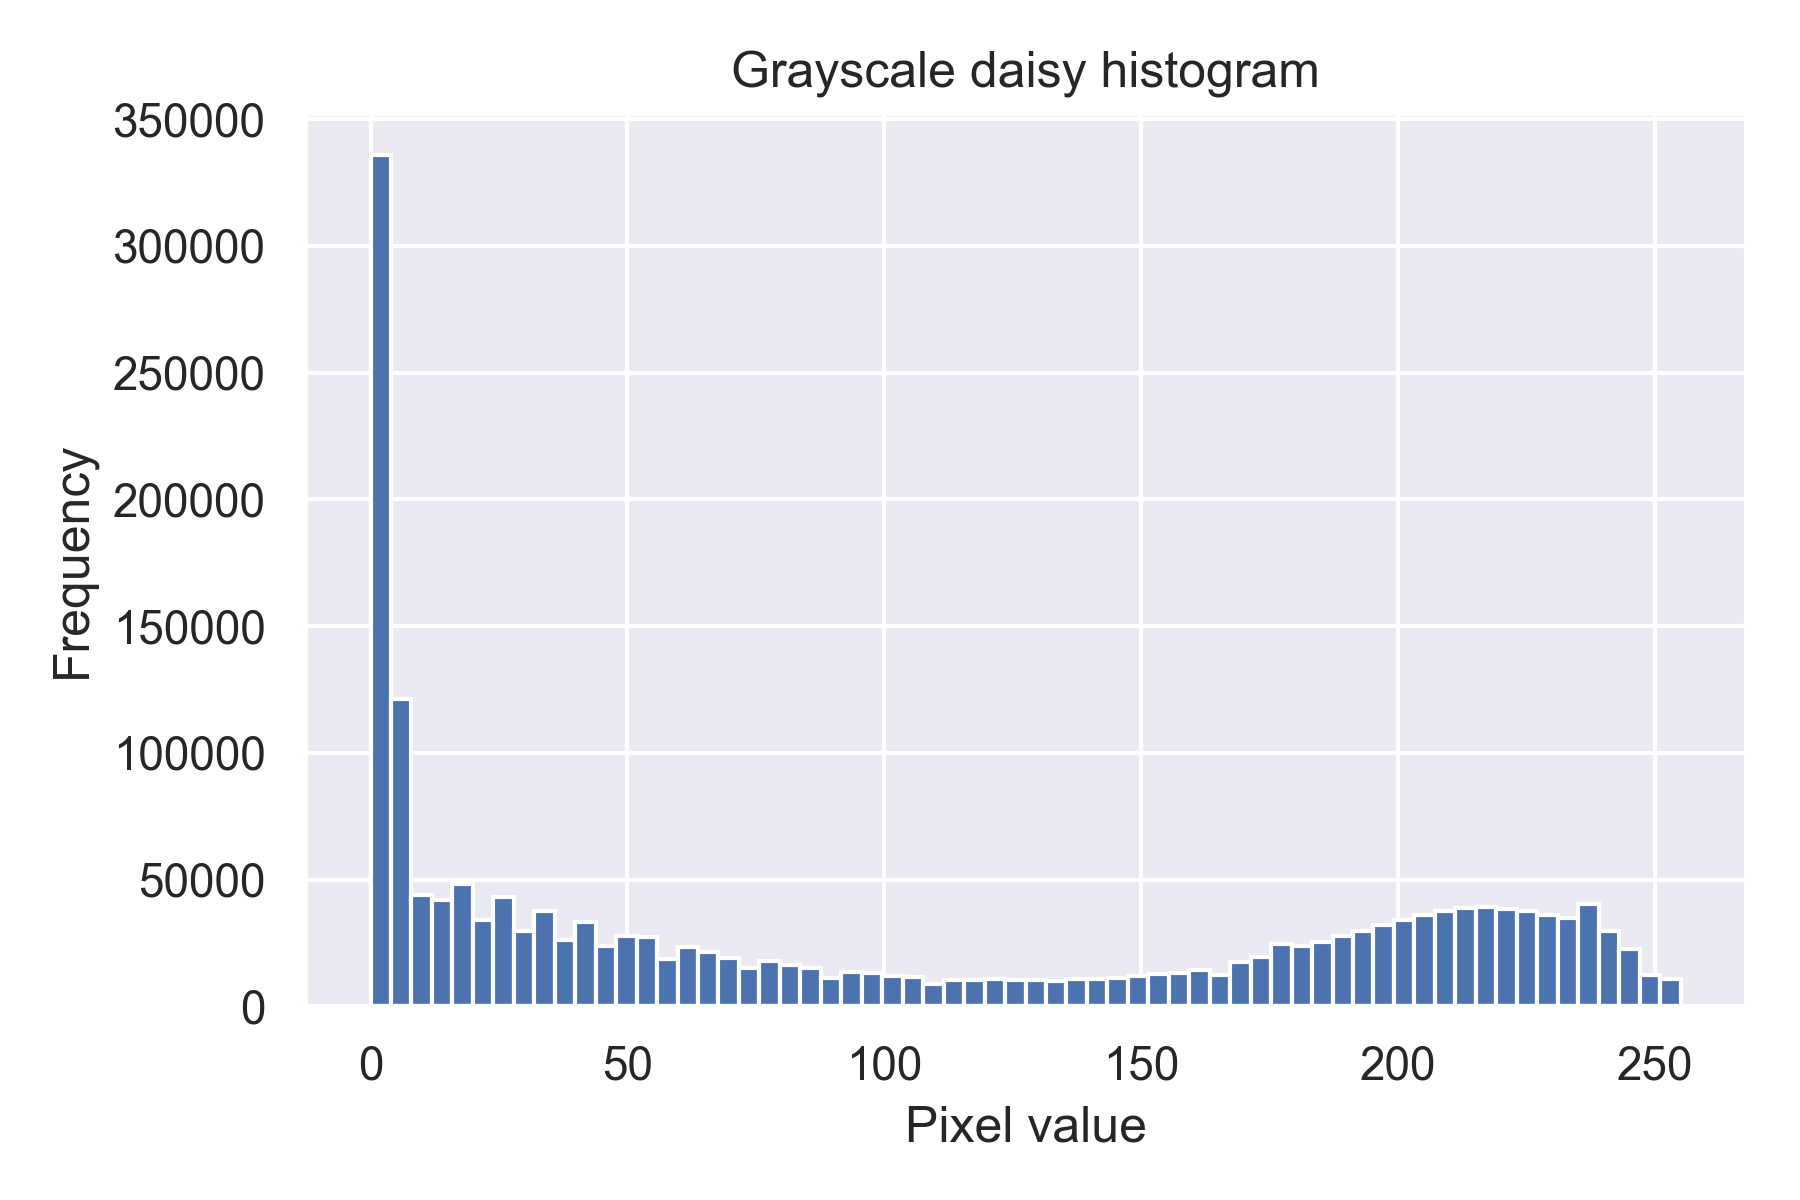
\includegraphics[width=.5\textwidth]{dissertation/figures/grayscale_histogram.png}
    \end{subfigure}
    \begin{subfigure}{0.5\textwidth}
        \centering
        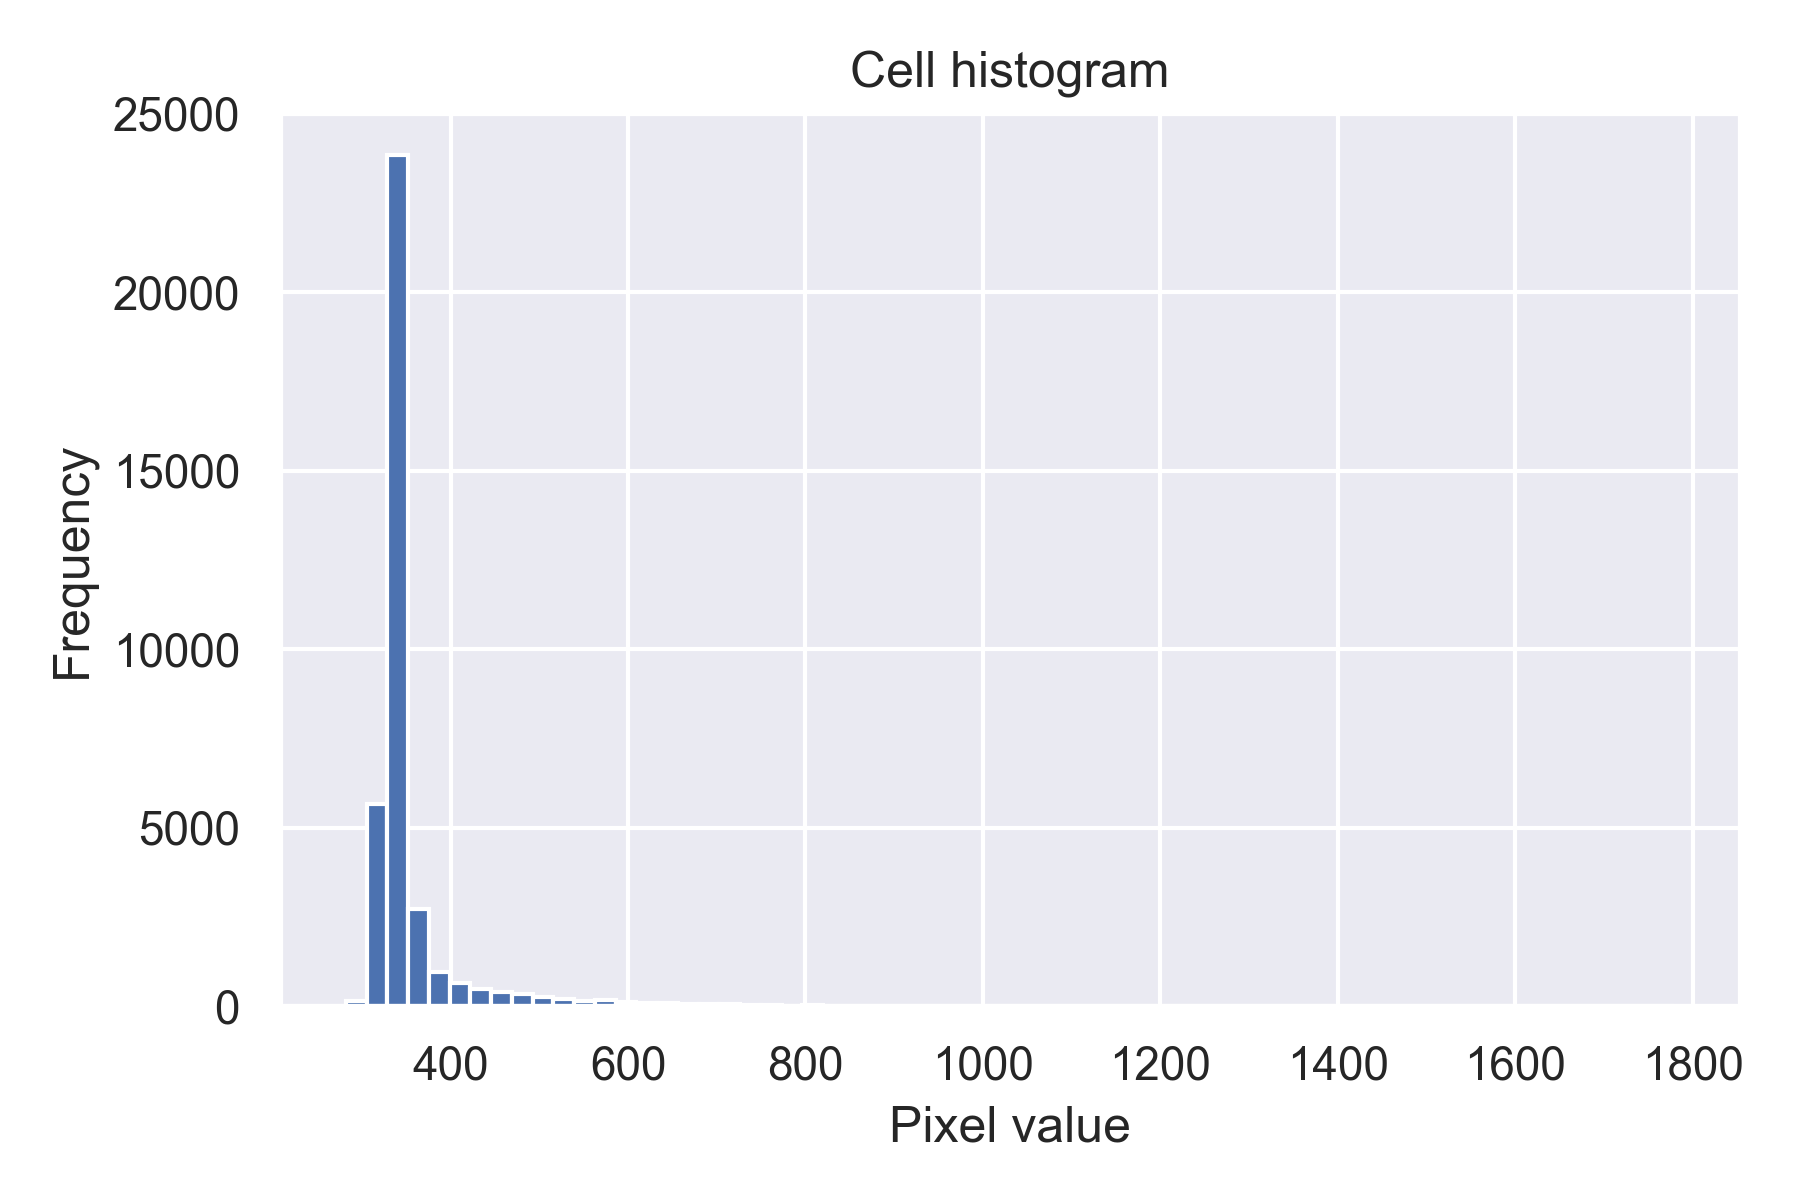
\includegraphics[width=.45\textwidth]{dissertation/figures/cell_histogram.png}
    \end{subfigure}
    \caption{Example images and their histogram. As we can see the grayscale image of lillies has two peaks of frequency.}
    \label{fig:thresholdhist}
\end{figure}
As such, we had to identify an alternative for a threshold. First, we selected the mean pixel value as the threshold. This yielded acceptable results, however some noisy pixels still came through the mask (see Figure \ref{fig:thresholdmean}). To fix that problem, the threshold value was set as the sum of the mean pixel value and the standard deviation. This decision was based on the hypothesis that the noise level of an image with a flat structure can be estimated from its variation. Results were satisfactory, as shown in Figure \ref{fig:thresholdstd}.

\begin{figure}[h]
    \centering
    \begin{subfigure}[h!]{0.4\textwidth}
        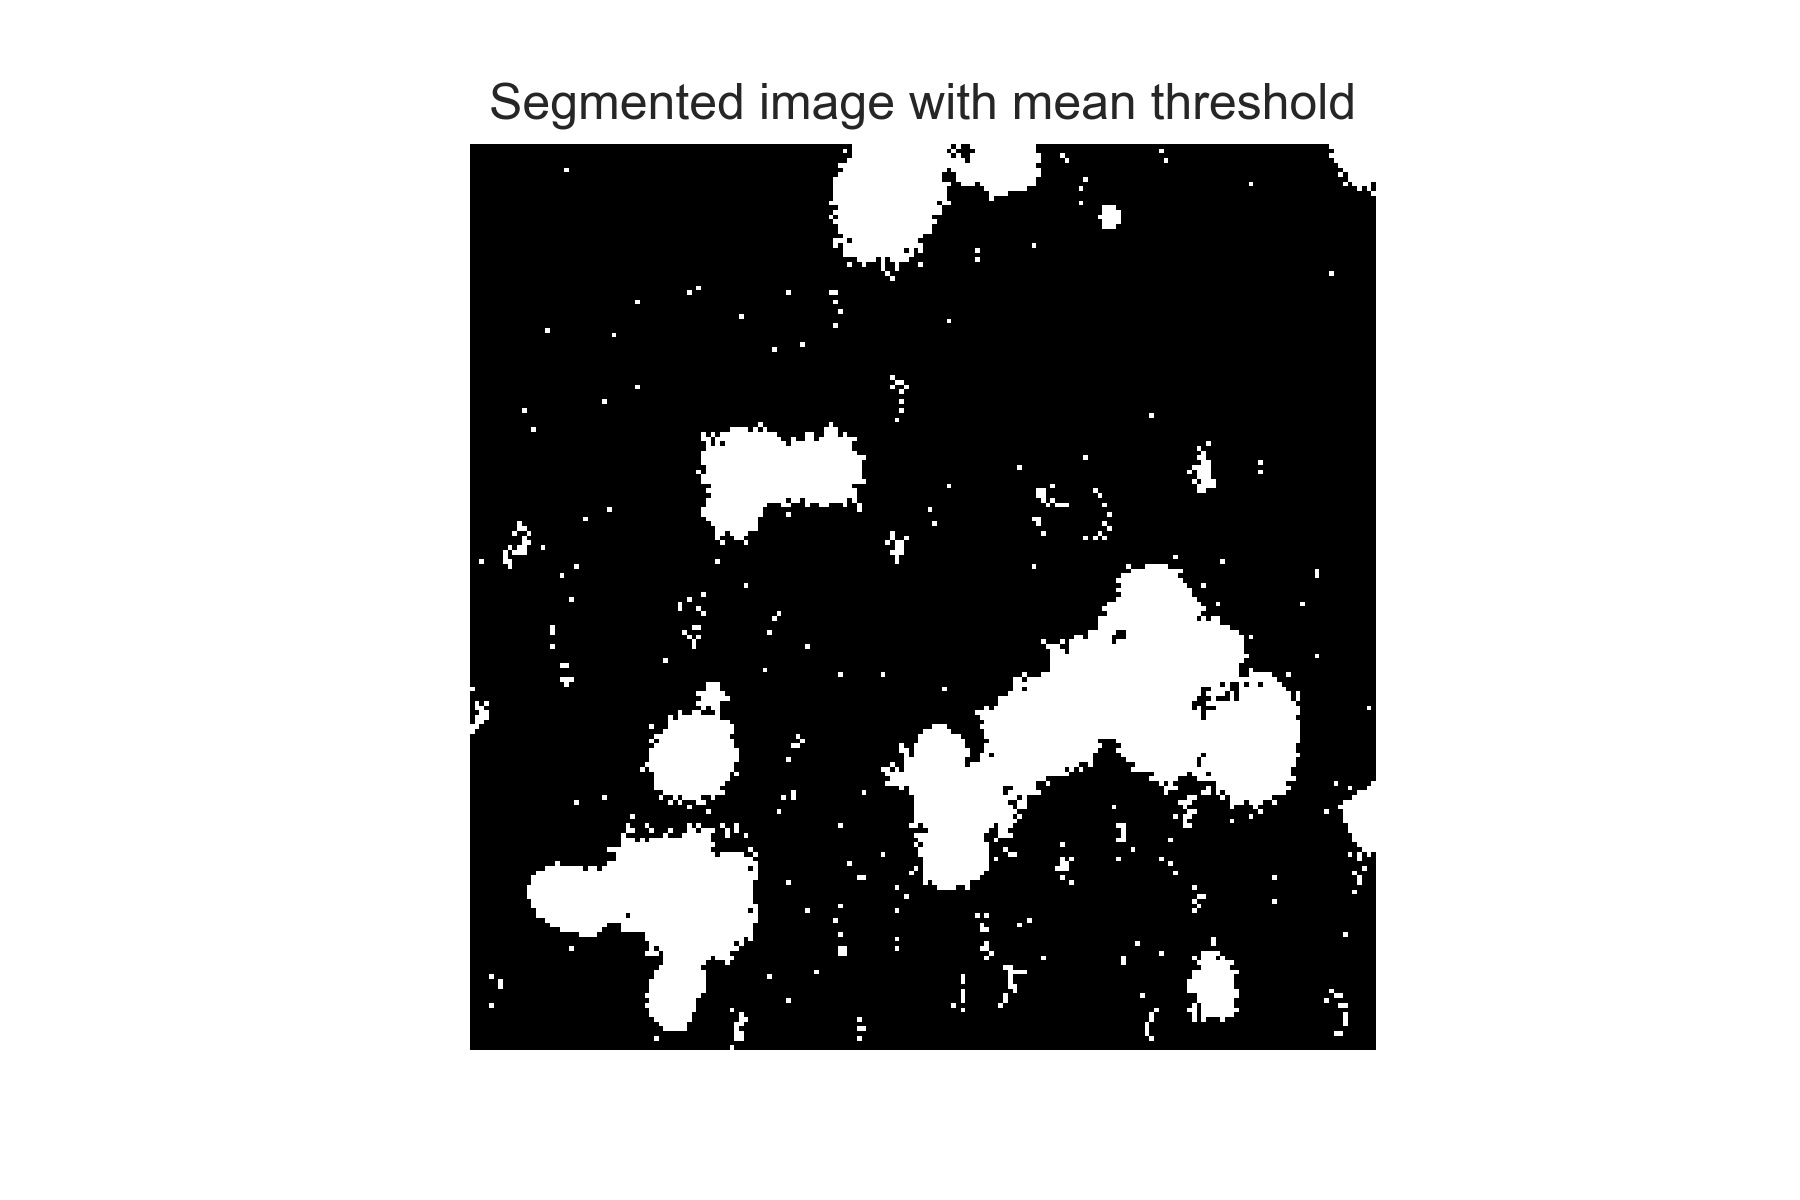
\includegraphics[width=\textwidth]{dissertation/figures/mean_threshold_cell.jpg}
        \caption{Threshold: mean pixel value}
        \label{fig:thresholdmean}
    \end{subfigure}
    \begin{subfigure}[h!]{0.4\textwidth}
        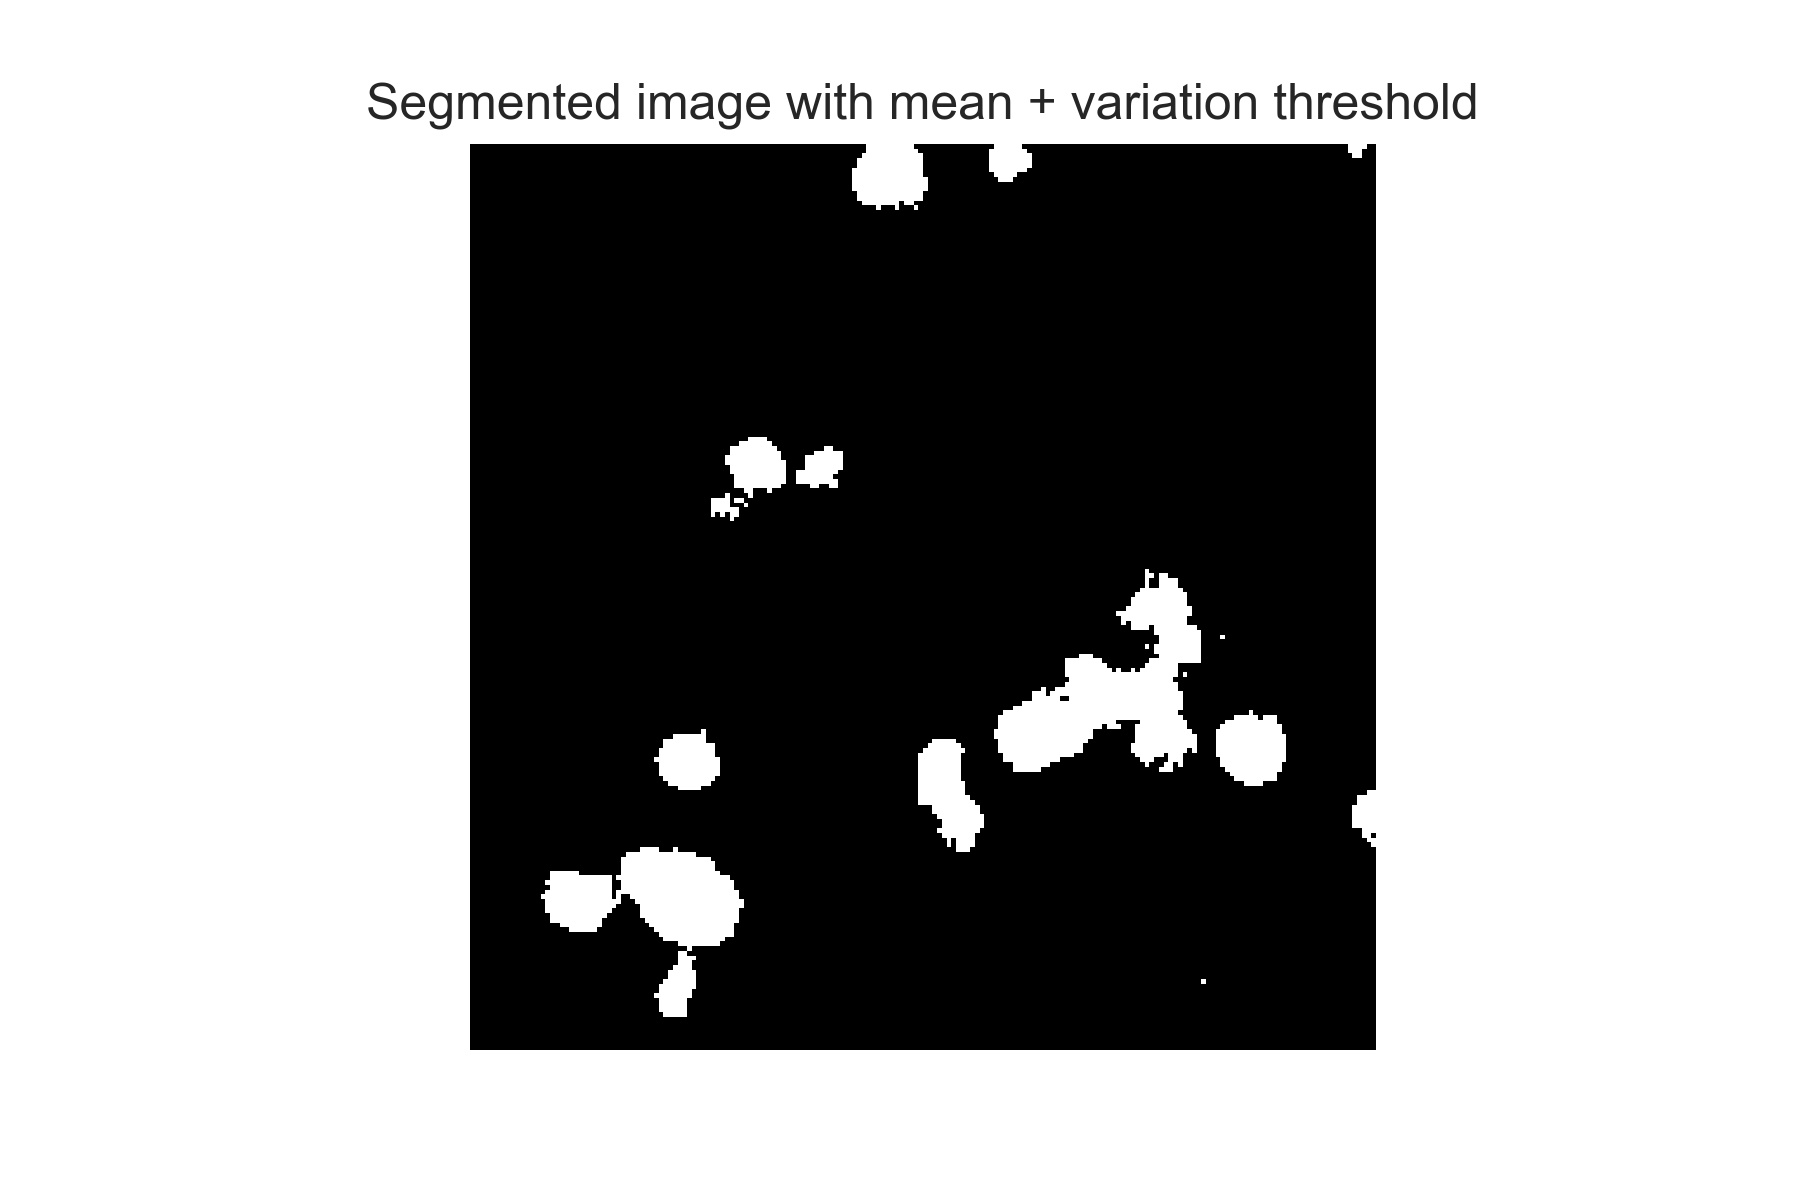
\includegraphics[width=\textwidth]{dissertation/figures/mean_std_threshold_cell.jpg}
        \caption{Threshold: mean + standard deviation}
        \label{fig:thresholdstd}
    \end{subfigure}
    \caption{Segmented images according to different threshold values.}
\end{figure}

%\subsection{Image masks for background correction}

%As mentioned in Section \ref{subsec:correction}, the microscope images of immune cells might have noise, especially in the background. Particularly in biomedical data, there has been research on background correction. Rather than fixing the background, we can evaluate whether removing the background entirely helps in this case by evaluating both masked and unmasked images.

\section{Convolutional autoencoder}

The main tool to be developed to exploit this dataset was a convolutional autoencoder. The autoencoder was built for two purposes: obtaining a smaller "code" representing each of the images to be fed into high-dimensional visualisation algorithms, and to be the starting block for a deep regression model.

\subsection{Structure}

The autoencoder was built using Keras \footnote{https://keras.io} for Python. We based our architecture off the standard Convolution --> Activation --> Pooling sequence of operations commonly used in convolutional neural networks (ref). The aim was to maximise the reduction of dimensionality while maintaining a satisfactory reconstructed image. Hence, the choice of number of hidden layers had to be made as a compromise.

The autoencoder was tuned by evaluation on a training and validation dataset. Its structure was established through both literature review and trial and error. The choice of hidden layer activation is PReLU, because of its evidenced benefit in improved loss (ref), as well as showing slightly better results in training. Moreover, convolutional layer sizes were kept quite high, instead making the neural network deeper to reduce dimension. Strides are used in the last layer instead of max pooling (why?) because results were slightly better. The choice of feature maps being higher in earlier layers comes from the encoded representation being smaller this way, as well as differences with the reversed being marginal. Finally, the output layer activation is sigmoid, as we are trying to predict a value between 0 and 1, as the images have been normalised. 

\subsection{Deep regression}

The regression model was built on the encoder layers of the autoencoder. The structure of the regression layers of the model was kept simple. Only two fully connected layers are used, with a Dropout layer in between. Dropout has shown to make models more robust and prevent overfitting.
Both softplus and linear activations were tried for the regression model. The linear activation was accompanied with a kernel restriction on the keras model of non-negativity, as interaction cannot be negative. Softplus keeps its output values positive. The results were similar, however the linear function performed overall better.
